\subsection{Schaltkreis}
    \vspace{-1mm}
    \begin{minipage}{0.49\linewidth}
        \begin{footnotesize}
            \begin{center}
                \vspace{2mm}
                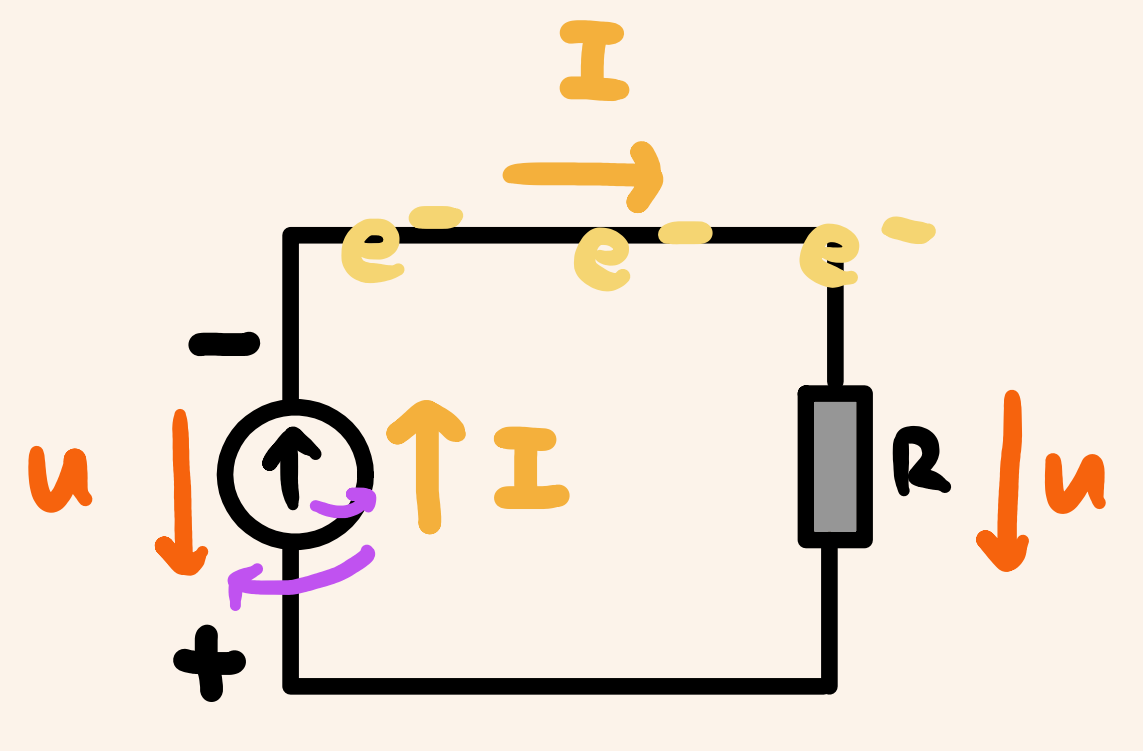
\includegraphics[width = 25mm]{src/images/schaltkreis.png}
            \end{center}
        \end{footnotesize}
    \end{minipage}
    \begin{minipage}{0.5\linewidth}
        \begin{scriptsize}
            \begin{center}
                \begin{align*}
                    \vec{I} = &\text{ Stromrichtung}
                    \\R = &\text{ Widerstand} 
                    \\\vec{U} = &\text{ Richtung des Spannungsabfall}
                    \\&\text{ Spannungsquelle: von mius nach plus}
                    \\&\text{ Widerstand: in Stromrichtung}
                \end{align*}
            \end{center}
        \end{scriptsize}
    \end{minipage}

    \subsubsection{Serieschaltung}
        \vspace{-1mm}
        \begin{minipage}{0.39\linewidth}
            \begin{footnotesize}
                \begin{center}
                    \vspace{2mm}
                    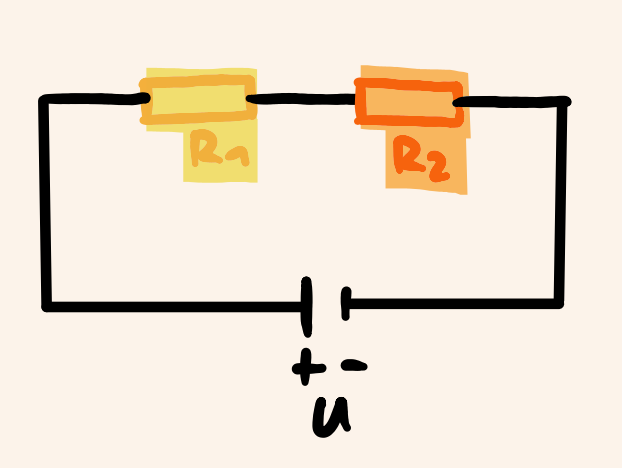
\includegraphics[width = 20mm]{src/images/serieschaltung.png}
                \end{center}
            \end{footnotesize}
        \end{minipage}
        \begin{minipage}{0.6\linewidth}
            \begin{scriptsize}
                \begin{center}
                    \begin{align*}
                        \text{Ladung:} \; Q_{\text{ges}} &= Q_i\\
                        \text{Stromstärke:} \; I_{\text{ges}} &= I_i\\
                        \text{Spannung:} \; U_{\text{ges}} &= \sum\limits_i U_i\\
                        \text{Widerstände:} \; R_{\text{res}} &= \sum\limits_i R_i\\
                        \text{Kondensatoren:} \; \frac{1}{C_{\text{res}}} &= \sum\limits_i \frac{1}{C_i}\\
                        \text{zwei Kondensatoren:} \; C_{res} &= \frac{C_1 \cdot C_2}{C_1 + C_2}
                    \end{align*}
                \end{center}
            \end{scriptsize}
        \end{minipage}
        \vspace{1mm}

    \subsubsection{Parallelschaltung}
        \vspace{-1mm}
        \begin{minipage}{0.39\linewidth}
            \begin{footnotesize}
                \begin{center}
                    \vspace{2mm}
                    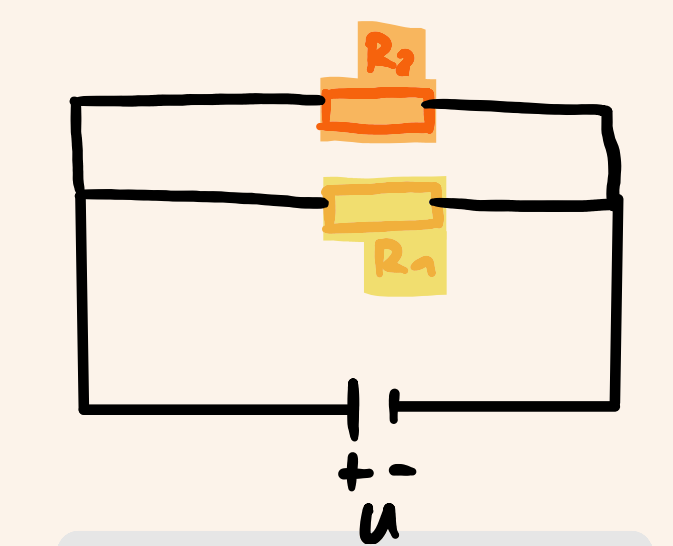
\includegraphics[width = 20mm]{src/images/parallelschaltung.png}
                \end{center}
            \end{footnotesize}
        \end{minipage}
        \begin{minipage}{0.6\linewidth}
            \begin{scriptsize}
                \begin{center}
                    \begin{align*}
                        \text{Ladung:} \; Q_{\text{ges}} &= \sum\limits_i Q_i\\
                        \text{Stromstärke:} \; I_{\text{ges}} &= \sum\limits_i I_i\\
                        \text{Spannung:} \; U_{\text{ges}} &= U_i\\
                        \text{Widerstände:} \; \frac{1}{R_{res}} &= \sum \frac{1}{R_i}\\
                        \text{zwei Widerstände:} \; R_{res} &= \frac{R_1 \cdot R_2}{R_1 + R_2}\\
                        \text{Kondensatoren:} \; C_{res} &= \sum\limits_i C_i
                    \end{align*}
                \end{center}
            \end{scriptsize}
        \end{minipage}